\documentclass[11pt,letterpaper]{report}
\usepackage[letterpaper,margin=2.5cm,headheight=15pt]{geometry}
\usepackage{fontspec}
\setmainfont{Segoe UI}
\usepackage[spanish,es-nodecimaldot]{babel}
\usepackage{xcolor}
\usepackage{graphicx}
\usepackage{booktabs}
\usepackage{tabularx}
\usepackage{longtable}
\usepackage{array}
\usepackage{enumitem}
\usepackage{fancyhdr}
\usepackage{hyperref}
\usepackage{tikz}
\usepackage{float}
\usepackage{caption}
\usepackage{microtype}
\newcommand{\University}{Universidad de las Fuerzas Armadas ESPE}
\newcommand{\Department}{Departamento de Ciencias de la Computación}
\newcommand{\Course}{Aseguramiento de la Calidad de Software}
\newcommand{\ReportTitle}{Medición de la Calidad en Uso mediante ISO/IEC 25022}
\newcommand{\ReportSubtitle}{Caso de estudio: MediSalud HIS}
\newcommand{\Authors}{Mesías Mariscal \\ Denise Rea \\ Julio Viche \\ Gabriel Murillo}
\newcommand{\AuthorsPlain}{Mesías Mariscal, Denise Rea, Julio Viche, Gabriel Murillo}
\newcommand{\NRC}{30733}
\newcommand{\Location}{Sangolquí, Ecuador}
\newcommand{\ReportDate}{2026}


\definecolor{mediteal}{HTML}{0C695F}
\definecolor{medidark}{HTML}{173F3B}
\definecolor{medicoral}{HTML}{D45D4C}
\definecolor{medigold}{HTML}{D59622}
\definecolor{medilight}{HTML}{F2F5F4}
\definecolor{medigrey}{HTML}{657B78}
\hypersetup{colorlinks=true,linkcolor=mediteal,urlcolor=medicoral,citecolor=mediteal,pdftitle={\ReportTitle}}
\setlength{\parindent}{0pt}
\setlength{\parskip}{6pt}
\setlist{nosep,leftmargin=*}
\renewcommand{\arraystretch}{1.2}
\pagestyle{fancy}
\fancyhf{}
\fancyhead[L]{\small MediSalud HIS}
\fancyhead[R]{\small ISO/IEC 25022}
\fancyfoot[C]{\thepage}

\newcommand{\sourcebadge}[1]{\par\smallskip\noindent\colorbox{medilight}{\parbox{0.95\textwidth}{\small\textbf{Trazabilidad:} #1}}\par\smallskip}
\newcommand{\statusgreen}{\textcolor{mediteal}{\textbf{VERDE}}}
\newcommand{\statusyellow}{\textcolor{medigold}{\textbf{AMARILLO}}}
\newcommand{\statusred}{\textcolor{medicoral}{\textbf{ROJO}}}

\begin{document}
\begin{titlepage}
\begin{tikzpicture}[remember picture,overlay]
  \fill[medidark] (current page.north west) rectangle ([xshift=5.0cm]current page.south west);
  \fill[mediteal] ([xshift=5.0cm]current page.north west) rectangle ([yshift=-1.0cm]current page.north east);
  \fill[medicoral] ([yshift=1.1cm]current page.south west) rectangle (current page.south east);
  \draw[medigold,line width=3pt] ([xshift=5.5cm,yshift=-1.8cm]current page.north west) -- ([xshift=-1.2cm,yshift=-1.8cm]current page.north east);
  \node[anchor=north west,text=white,align=left,text width=3.4cm] at ([xshift=1.0cm,yshift=-2.0cm]current page.north west) {\Large\bfseries ESPE\\[0.35cm]\small Universidad de las Fuerzas Armadas\\[0.25cm]\footnotesize Departamento de\\Ciencias de la\\Computación};
  \node[anchor=south east,text=white] at ([xshift=-1.0cm,yshift=0.38cm]current page.south east) {\large\bfseries \Location\quad |\quad \ReportDate};
\end{tikzpicture}
\color{medidark}\vspace*{5.1cm}
\hspace*{4.8cm}\begin{minipage}{0.64\textwidth}
{\color{mediteal}\small\bfseries TALLER GUIADO INTEGRAL}\par\vspace{0.3cm}
{\fontsize{25}{30}\selectfont\bfseries Medición de la Calidad en Uso\\[0.1cm]mediante ISO/IEC 25022}\par\vspace{0.35cm}
{\Large\color{medicoral}\ReportSubtitle}\par\vspace{0.8cm}
{\large\bfseries\Course}\par\vspace{1cm}
\begin{tabular}{@{}ll@{}}
\textbf{Integrantes} & \begin{tabular}[t]{@{}l@{}}\Authors\end{tabular}\\[0.5cm]
\textbf{NRC} & \NRC
\end{tabular}
\end{minipage}
\vfill
\end{titlepage}

\pagenumbering{roman}
\chapter*{Resumen ejecutivo}
Este informe evalúa la calidad en uso de MediSalud HIS con el marco ISO/IEC 25022. Se preservaron 3.000 incidentes del caso académico y se generaron, con semilla 25022, 6.000 eventos y 2.000 encuestas ficticias para 2025. La automatización produjo diez métricas: tres verdes, cuatro amarillas y tres rojas. Los principales riesgos son los incidentes de privacidad, los errores de facturación y las recetas incorrectas.

La aplicación local reproduce defectos controlados sin introducir vulnerabilidades reales. El propósito no es mejorar el sistema durante la medición, sino observar tareas, registrar evidencia y formular un plan posterior.

\tableofcontents
\listoftables
\listoffigures
\clearpage
\pagenumbering{arabic}

\chapter{Escenario 1: caso empresarial MediSalud}
\sourcebadge{Actividad desarrollada literalmente desde el Documento Padre, escenario 1.}

MediSalud Ecuador opera un HIS con procesos de agendamiento, admisión, historia clínica electrónica (HCE), prescripción, farmacia, facturación, telemedicina y reportes gerenciales. La problemática no es únicamente disponibilidad técnica: los usuarios encuentran lentitud, abandonos, duplicidades y riesgos que afectan objetivos reales.

\begin{table}[H]\centering
\caption{Matriz de análisis inicial}
\begin{tabularx}{\textwidth}{>{\bfseries}p{0.31\textwidth}X}
\toprule
Pregunta & Respuesta del equipo\\\midrule
Procesos más críticos & Atención y registro de HCE; facturación y seguros; agendamiento y admisión.\\
Usuarios más afectados & Médicos tratantes, pacientes y personal de admisión.\\
Evidencia disponible & Quejas, incidentes y disponibilidad de servidores.\\
Evidencia faltante & Éxito de tareas, tiempos reales, errores, satisfacción y variación por contexto.\\\bottomrule
\end{tabularx}
\end{table}

La evaluación se concentra en la experiencia observable y no utiliza métricas internas del código como sustituto de la calidad en uso.


\chapter{Escenario 2: clasificación ISO/IEC 25022}
\sourcebadge{Actividad desarrollada literalmente desde el Documento Padre, escenario 2. El detalle completo está en el CSV procesado.}

Se aplicó una clasificación determinista con precedencia de libertad de riesgo. Esta precedencia evita etiquetar como simple fallo funcional un evento con posibles consecuencias clínicas, financieras o de privacidad.

\begin{table}[H]\centering
\caption{Distribución de 3.000 incidentes}
\begin{tabular}{lrr}\toprule
Característica & Cantidad & Porcentaje\\\midrule
Efectividad & 1.853 & 61,77\%\\
Libertad de riesgo & 359 & 11,97\%\\
Eficiencia & 347 & 11,57\%\\
Cobertura de contexto & 339 & 11,30\%\\
Satisfacción & 102 & 3,40\%\\\bottomrule
\end{tabular}
\end{table}

Por ejemplo, ``el historial de alergias no carga'' se clasifica como libertad de riesgo: aunque la tarea falla, la consecuencia principal puede ser una decisión clínica insegura. Cada registro conserva la regla coincidente y una justificación técnica auditable.


\chapter{Escenario 3: modelo SQuaRE}
\sourcebadge{Actividad desarrollada literalmente desde el Documento Padre, escenario 3.}

La calidad interna observa código y arquitectura; la externa observa el comportamiento en pruebas; y la calidad en uso observa a usuarios que intentan alcanzar objetivos dentro de un contexto. Son perspectivas relacionadas, pero no intercambiables.

\begin{table}[H]\centering
\caption{Niveles de calidad aplicados a MediSalud}
\begin{tabularx}{\textwidth}{lX}\toprule
Nivel & Ejemplo\\\midrule
Interna & Complejidad y cobertura del módulo de facturación.\\
Externa & Prueba de carga del portal de citas con concurrencia controlada.\\
En uso & Tiempo real para registrar una nota durante consulta externa.\\\bottomrule
\end{tabularx}
\end{table}

\begin{figure}[H]\centering
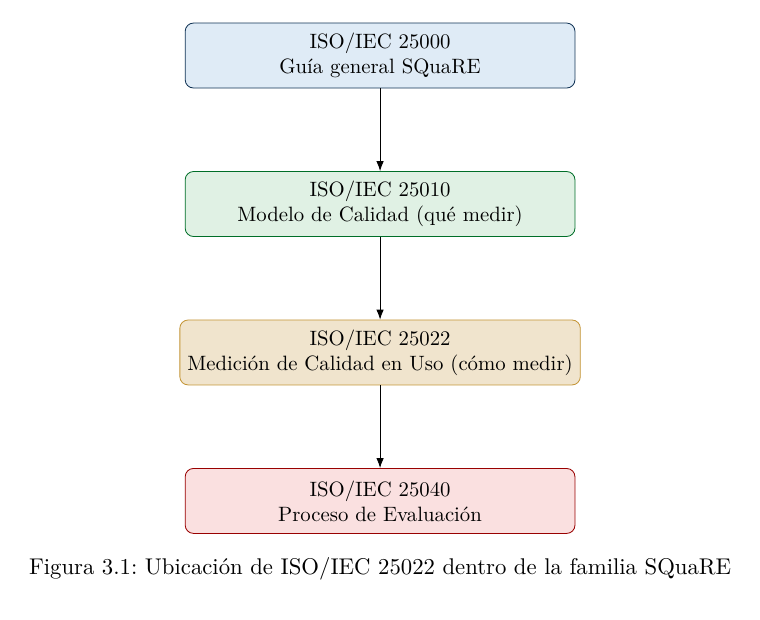
\includegraphics[width=0.62\textwidth]{figures/square.png}
\caption{Ubicación de ISO/IEC 25022 en la familia SQuaRE. Fuente: Documento Padre.}
\end{figure}


\chapter{Escenario 4: atributos de calidad en uso}
\sourcebadge{Reconstruido porque el material recibido solo incluye este escenario en el índice.}

Los atributos observables se definieron alrededor de tareas: completitud y exactitud del resultado, tiempo de tarea, recursos consumidos, confianza, comodidad, prevención de daños y adaptación a sedes, horarios, dispositivos y conectividad.

\begin{table}[H]\centering
\caption{Atributos priorizados}
\begin{tabularx}{\textwidth}{lXl}\toprule
Característica & Atributos observables & Contexto\\\midrule
Efectividad & Éxito, exactitud, completitud & Citas, HCE y recetas\\
Eficiencia & Tiempo y esfuerzo & HCE e imagenología\\
Satisfacción & Confianza, utilidad y comodidad & Portal y aplicación móvil\\
Libertad de riesgo & Riesgo clínico, financiero y privacidad & Atención y facturación\\
Cobertura & Adaptación y consistencia & Sedes, horarios y conectividad\\\bottomrule
\end{tabularx}
\end{table}


\chapter{Escenario 5: mapeo de características}
\sourcebadge{Reconstruido desde el índice y la metodología transversal del caso.}

\begin{longtable}{p{0.22\textwidth}p{0.22\textwidth}p{0.25\textwidth}p{0.20\textwidth}}
\caption{Tareas, usuarios y características}\\\toprule
Tarea & Usuario & Evidencia & Característica\\\midrule\endfirsthead
\toprule Tarea & Usuario & Evidencia & Característica\\\midrule\endhead
Guardar nota HCE & Médico & Duración y resultado & Eficiencia / efectividad\\
Agendar cita & Paciente & Pasos, éxito y abandono & Efectividad / satisfacción\\
Emitir factura & Admisión & Duplicidad y error & Libertad de riesgo\\
Completar teleconsulta & Paciente & Caídas y finalización & Cobertura de contexto\\
Dispensar receta & Farmacia & Dosis y alertas & Libertad de riesgo\\
Consultar indicadores & Gerencia & Filtros y trazabilidad & Efectividad\\\bottomrule
\end{longtable}

\chapter{Escenario 6: diseño de métricas}
\sourcebadge{Reconstruido desde el índice. Las metas RNF-01, RNF-03, RNF-04 y RNF-05 provienen del caso.}

\begin{longtable}{llll}
\caption{Catálogo resumido de métricas}\\\toprule
Código & Métrica & Unidad & Meta\\\midrule\endfirsthead
\toprule Código & Métrica & Unidad & Meta\\\midrule\endhead
M-EFI-01 & P90 registro HCE & segundos & $\leq 8$\\
M-EFE-01 & Éxito de agendamiento & \% & $\geq 95$\\
M-RIE-01 & Errores de facturación & \% & $<1$\\
M-SAT-01 & Abandono móvil & \% & $<10$\\
M-CC-01 & Variabilidad HCE entre sedes & segundos & $\leq 2$\\
M-RIE-02 & Incidentes de privacidad & conteo & 0\\
M-SAT-02 & CSAT promedio & 1--5 & $\geq 4$\\
M-EFE-02 & Recetas correctas & \% & 100\\
M-EFI-02 & P90 carga de imagen & segundos & $\leq 10$\\
M-CC-02 & Caídas de teleconsulta & \% & $<5$\\\bottomrule
\end{longtable}

Cada métrica mantiene fuente, fórmula, meta y umbrales de semáforo dentro del catálogo versionado.

\chapter{Escenario 7: obtención de datos}
\sourcebadge{Reconstruido desde el índice; los datos adicionales son ficticios y se identifican como simulados.}

La fuente original contiene 3.000 incidentes. Su copia de trabajo fue verificada con SHA-256. El valor se presenta en dos segmentos para conservar la legibilidad:

\begin{center}\small\ttfamily
814F3E5D8CF983A86BC125EC9C8461E\\
3728C91DDCE1CFE8A5518ABD7A53CDC17
\end{center}

El archivo no se modifica durante el pipeline.

La simulación con semilla 25022 produce 6.000 eventos y 2.000 encuestas entre enero y diciembre de 2025. Cada evento contiene fecha, sede, rol, módulo, duración, resultado, código de error, característica ISO, semilla y bandera \texttt{simulated}.

\begin{figure}[H]\centering
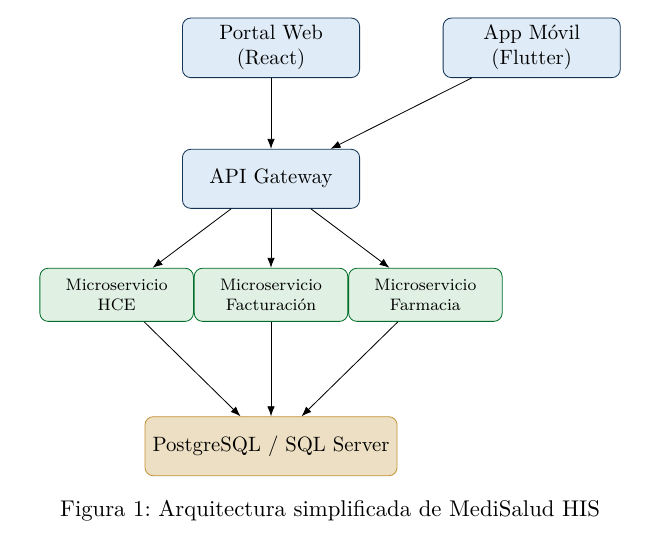
\includegraphics[width=0.9\textwidth]{figures/architecture.png}
\caption{Arquitectura simplificada del caso. Fuente: Documento Padre.}
\end{figure}

\chapter{Escenario 8: automatización de la medición}
\sourcebadge{Reconstruido desde el índice y ejecutado mediante el paquete Python \texttt{analytics}.}

El flujo separa clasificación, simulación, cálculo y exportación. La ejecución usa una semilla explícita, escribe únicamente archivos derivados y conserva manifiestos con periodo y procedencia.

\begin{enumerate}
\item Leer el dataset original sin modificarlo.
\item Clasificar incidentes con precedencia de riesgo.
\item Generar eventos y encuestas reproducibles.
\item Calcular las diez métricas.
\item Exportar CSV y JSON para API, tablero e informe.
\end{enumerate}

Las pruebas verifican casos de riesgo, eficiencia, percentiles y repetibilidad de la semilla.


\chapter{Escenario 9: indicadores KPI}
\sourcebadge{Reconstruido desde el índice. Valores producidos por la ejecución reproducible con semilla 25022.}

\begin{longtable}{llrl}
\caption{Resultados del tablero}\\\toprule
Código & Indicador & Valor & Estado\\\midrule\endfirsthead
\toprule Código & Indicador & Valor & Estado\\\midrule\endhead
M-EFI-01 & P90 registro HCE & 11,71 s & \statusyellow\\
M-EFE-01 & Éxito de agendamiento & 87,86\% & \statusyellow\\
M-RIE-01 & Errores de facturación & 4,50\% & \statusred\\
M-SAT-01 & Abandono móvil & 9,80\% & \statusgreen\\
M-CC-01 & Variabilidad por sede & 0,61 s & \statusgreen\\
M-RIE-02 & Incidentes de privacidad & 41 & \statusred\\
M-SAT-02 & CSAT promedio & 3,42 & \statusyellow\\
M-EFE-02 & Recetas correctas & 96,52\% & \statusred\\
M-EFI-02 & P90 carga de imagen & 9,42 s & \statusgreen\\
M-CC-02 & Caídas de teleconsulta & 8,68\% & \statusyellow\\\bottomrule
\end{longtable}

El balance general es tres verdes, cuatro amarillos y tres rojos. Los colores no reemplazan el valor ni su meta: ambos permanecen visibles para evitar interpretaciones aisladas.

\chapter{Escenario 10: interpretación de resultados}
\sourcebadge{Reconstruido desde el índice; interpretación basada en las salidas de la simulación.}

La HCE incumple el percentil 90 aunque la variación entre sedes permanece controlada; el patrón apunta a las horas pico más que a una sede aislada. El agendamiento presenta una brecha de 7,14 puntos porcentuales respecto de la meta. La facturación cuadruplica el límite del 1\% y exige prioridad por impacto financiero.

Los 41 incidentes de privacidad y el 3,48\% de recetas simuladas incorrectas son hallazgos de riesgo. La carga de imagen cumple, pero las caídas de teleconsulta superan la meta. La satisfacción media tampoco alcanza el objetivo, aunque el abandono de encuesta se mantiene bajo el umbral.

No se infiere causalidad definitiva a partir de correlaciones. Las recomendaciones requieren observar trazas, contexto y tarea antes de intervenir.


\chapter{Escenario 11: presentación ejecutiva}
\sourcebadge{Reconstruido desde el índice para la Dirección General de MediSalud.}

\textbf{Decisión solicitada.} Priorizar un programa trimestral de calidad en uso que atienda primero privacidad, prescripción y facturación; después desempeño HCE, citas y telemedicina.

\begin{table}[H]\centering
\caption{Resumen para dirección}
\begin{tabularx}{\textwidth}{lXl}\toprule
Prioridad & Evidencia & Resultado\\\midrule
Crítica & 41 incidentes de privacidad & Riesgo clínico y regulatorio\\
Crítica & 4,50\% de errores de facturación & Supera meta de 1\%\\
Crítica & 96,52\% de recetas correctas & No admite tolerancia clínica\\
Alta & HCE P90 de 11,71 segundos & Supera meta de 8 segundos\\
Alta & 8,68\% de caídas de teleconsulta & No alcanza 95\% de finalización\\\bottomrule
\end{tabularx}
\end{table}

La evidencia procede de un laboratorio académico y debe validarse en un entorno institucional antes de adoptar decisiones productivas.


\chapter{Escenario 12: plan de mejora continua}
\sourcebadge{Reconstruido desde el índice. Las mejoras se proponen, pero no se aplican a la línea base simulada.}

\begin{longtable}{p{0.16\textwidth}p{0.34\textwidth}p{0.27\textwidth}p{0.12\textwidth}}
\caption{Ciclo de mejora propuesto}\\\toprule
Fase & Acción & Evidencia de cierre & Plazo\\\midrule\endfirsthead
\toprule Fase & Acción & Evidencia de cierre & Plazo\\\midrule\endhead
Planificar & Revisar accesos, reglas clínicas y duplicidad financiera & Riesgos y responsables aprobados & 30 días\\
Hacer & Probar controles en entorno aislado & Pruebas de tarea y regresión & 60 días\\
Verificar & Repetir métricas con igual contexto & Comparación antes/después & 90 días\\
Actuar & Estandarizar controles que cumplan metas & Reporte trimestral & Continuo\\\bottomrule
\end{longtable}

La línea base queda congelada mediante semilla y manifiesto. Una mejora posterior deberá ejecutarse en otra versión y nunca sobrescribir la evidencia inicial.

\chapter{Reto final integrador}
\sourcebadge{Reconstruido desde el índice del reto integrador.}

El reto conecta los elementos del caso en una cadena verificable:

\begin{center}
\textbf{Problema} $\rightarrow$ \textbf{Usuario y tarea} $\rightarrow$ \textbf{Evento} $\rightarrow$ \textbf{Característica ISO} $\rightarrow$ \textbf{Métrica} $\rightarrow$ \textbf{Resultado} $\rightarrow$ \textbf{Riesgo} $\rightarrow$ \textbf{Recomendación}
\end{center}

Para la facturación duplicada, el usuario es admisión, la tarea es emitir una factura, el evento es \texttt{SIM-BILL-DUP}, la característica es libertad de riesgo y la métrica M-RIE-01 resulta 4,50\% frente a una meta menor al 1\%. El riesgo es financiero y la recomendación es probar idempotencia y conciliación en una iteración posterior, sin alterar la línea base.

La misma estructura se aplica a HCE, citas, prescripción, imagenología y telemedicina. Esto permite defender cada conclusión con una fuente concreta y evita recomendaciones basadas únicamente en percepción.



\begin{thebibliography}{9}
\bibitem{iso25022} ISO/IEC. \textit{ISO/IEC 25022:2016 Systems and software engineering -- Systems and software quality requirements and evaluation (SQuaRE) -- Measurement of quality in use}. 2016.
\bibitem{iso25010} ISO/IEC. \textit{ISO/IEC 25010 Systems and software Quality Requirements and Evaluation -- Product quality model}. 2011.
\bibitem{taller} Material docente. \textit{Taller Guiado Integral: Medición de la Calidad en Uso mediante ISO/IEC 25022. Caso MediSalud Ecuador}. Versión parcial suministrada.
\end{thebibliography}

\appendix
\chapter{Artefactos reproducibles}
El dataset original se conserva en \texttt{data/original}; los generadores están en \texttt{analytics}; los contratos en \texttt{contracts}; y las evidencias seleccionadas en \texttt{evidencias}. El CSV completo de clasificación se entrega como archivo separado para mantener legible este informe.
\end{document}
